% Created by tikzDevice version 0.12 on 2019-03-27 16:15:24
% !TEX encoding = UTF-8 Unicode
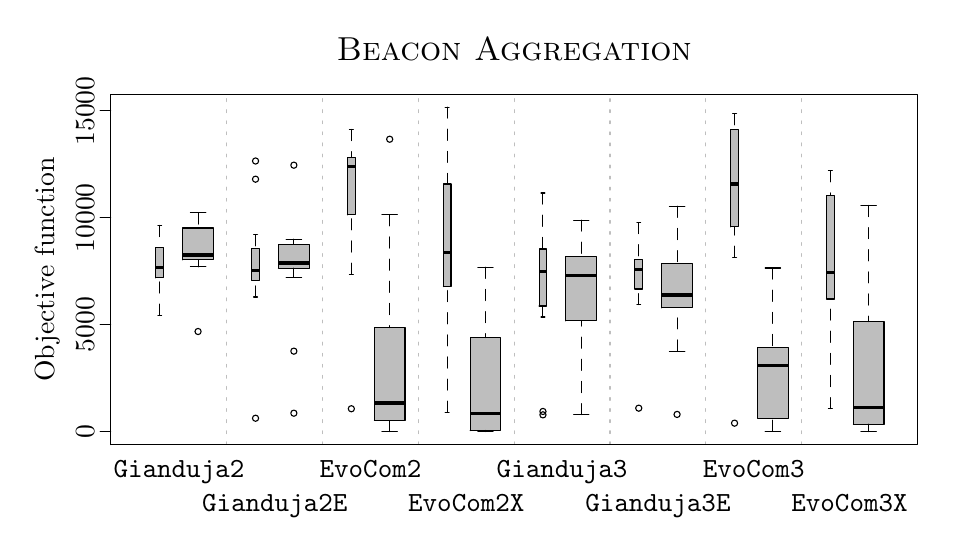
\begin{tikzpicture}[x=1pt,y=1pt]
\definecolor{fillColor}{RGB}{255,255,255}
\path[use as bounding box,fill=fillColor,fill opacity=0.00] (0,0) rectangle (325.21,180.67);
\begin{scope}
\path[clip] ( 30.00, 30.00) rectangle (321.61,156.67);
\definecolor{fillColor}{RGB}{190,190,190}

\path[fill=fillColor] ( 46.34, 90.29) --
	( 49.11, 90.29) --
	( 49.11,101.38) --
	( 46.34,101.38) --
	cycle;
\definecolor{drawColor}{RGB}{0,0,0}

\path[draw=drawColor,line width= 1.2pt,line join=round] ( 46.34, 94.09) -- ( 49.11, 94.09);

\path[draw=drawColor,line width= 0.4pt,dash pattern=on 4pt off 4pt ,line join=round,line cap=round] ( 47.72, 76.80) -- ( 47.72, 90.29);

\path[draw=drawColor,line width= 0.4pt,dash pattern=on 4pt off 4pt ,line join=round,line cap=round] ( 47.72,109.17) -- ( 47.72,101.38);

\path[draw=drawColor,line width= 0.4pt,line join=round,line cap=round] ( 47.03, 76.80) -- ( 48.42, 76.80);

\path[draw=drawColor,line width= 0.4pt,line join=round,line cap=round] ( 47.03,109.17) -- ( 48.42,109.17);

\path[draw=drawColor,line width= 0.4pt,line join=round,line cap=round] ( 46.34, 90.29) --
	( 49.11, 90.29) --
	( 49.11,101.38) --
	( 46.34,101.38) --
	( 46.34, 90.29);

\path[fill=fillColor] ( 56.03, 96.78) --
	( 67.11, 96.78) --
	( 67.11,108.27) --
	( 56.03,108.27) --
	cycle;

\path[draw=drawColor,line width= 1.2pt,line join=round] ( 56.03, 98.49) -- ( 67.11, 98.49);

\path[draw=drawColor,line width= 0.4pt,dash pattern=on 4pt off 4pt ,line join=round,line cap=round] ( 61.57, 94.21) -- ( 61.57, 96.78);

\path[draw=drawColor,line width= 0.4pt,dash pattern=on 4pt off 4pt ,line join=round,line cap=round] ( 61.57,113.73) -- ( 61.57,108.27);

\path[draw=drawColor,line width= 0.4pt,line join=round,line cap=round] ( 58.80, 94.21) -- ( 64.34, 94.21);

\path[draw=drawColor,line width= 0.4pt,line join=round,line cap=round] ( 58.80,113.73) -- ( 64.34,113.73);

\path[draw=drawColor,line width= 0.4pt,line join=round,line cap=round] ( 56.03, 96.78) --
	( 67.11, 96.78) --
	( 67.11,108.27) --
	( 56.03,108.27) --
	( 56.03, 96.78);

\path[draw=drawColor,line width= 0.4pt,line join=round,line cap=round] ( 61.57, 70.88) circle (  1.12);

\path[fill=fillColor] ( 80.96, 89.41) --
	( 83.73, 89.41) --
	( 83.73,100.74) --
	( 80.96,100.74) --
	cycle;

\path[draw=drawColor,line width= 1.2pt,line join=round] ( 80.96, 92.97) -- ( 83.73, 92.97);

\path[draw=drawColor,line width= 0.4pt,dash pattern=on 4pt off 4pt ,line join=round,line cap=round] ( 82.34, 83.35) -- ( 82.34, 89.41);

\path[draw=drawColor,line width= 0.4pt,dash pattern=on 4pt off 4pt ,line join=round,line cap=round] ( 82.34,105.81) -- ( 82.34,100.74);

\path[draw=drawColor,line width= 0.4pt,line join=round,line cap=round] ( 81.65, 83.35) -- ( 83.03, 83.35);

\path[draw=drawColor,line width= 0.4pt,line join=round,line cap=round] ( 81.65,105.81) -- ( 83.03,105.81);

\path[draw=drawColor,line width= 0.4pt,line join=round,line cap=round] ( 80.96, 89.41) --
	( 83.73, 89.41) --
	( 83.73,100.74) --
	( 80.96,100.74) --
	( 80.96, 89.41);

\path[draw=drawColor,line width= 0.4pt,line join=round,line cap=round] ( 82.34, 39.54) circle (  1.12);

\path[draw=drawColor,line width= 0.4pt,line join=round,line cap=round] ( 82.34,125.92) circle (  1.12);

\path[draw=drawColor,line width= 0.4pt,line join=round,line cap=round] ( 82.34,132.49) circle (  1.12);

\path[fill=fillColor] ( 90.65, 93.79) --
	(101.73, 93.79) --
	(101.73,102.39) --
	( 90.65,102.39) --
	cycle;

\path[draw=drawColor,line width= 1.2pt,line join=round] ( 90.65, 95.64) -- (101.73, 95.64);

\path[draw=drawColor,line width= 0.4pt,dash pattern=on 4pt off 4pt ,line join=round,line cap=round] ( 96.19, 90.52) -- ( 96.19, 93.79);

\path[draw=drawColor,line width= 0.4pt,dash pattern=on 4pt off 4pt ,line join=round,line cap=round] ( 96.19,104.25) -- ( 96.19,102.39);

\path[draw=drawColor,line width= 0.4pt,line join=round,line cap=round] ( 93.42, 90.52) -- ( 98.96, 90.52);

\path[draw=drawColor,line width= 0.4pt,line join=round,line cap=round] ( 93.42,104.25) -- ( 98.96,104.25);

\path[draw=drawColor,line width= 0.4pt,line join=round,line cap=round] ( 90.65, 93.79) --
	(101.73, 93.79) --
	(101.73,102.39) --
	( 90.65,102.39) --
	( 90.65, 93.79);

\path[draw=drawColor,line width= 0.4pt,line join=round,line cap=round] ( 96.19, 41.36) circle (  1.12);

\path[draw=drawColor,line width= 0.4pt,line join=round,line cap=round] ( 96.19,130.98) circle (  1.12);

\path[draw=drawColor,line width= 0.4pt,line join=round,line cap=round] ( 96.19, 63.78) circle (  1.12);

\path[fill=fillColor] (115.57,113.03) --
	(118.34,113.03) --
	(118.34,133.86) --
	(115.57,133.86) --
	cycle;

\path[draw=drawColor,line width= 1.2pt,line join=round] (115.57,130.51) -- (118.34,130.51);

\path[draw=drawColor,line width= 0.4pt,dash pattern=on 4pt off 4pt ,line join=round,line cap=round] (116.96, 91.61) -- (116.96,113.03);

\path[draw=drawColor,line width= 0.4pt,dash pattern=on 4pt off 4pt ,line join=round,line cap=round] (116.96,143.89) -- (116.96,133.86);

\path[draw=drawColor,line width= 0.4pt,line join=round,line cap=round] (116.27, 91.61) -- (117.65, 91.61);

\path[draw=drawColor,line width= 0.4pt,line join=round,line cap=round] (116.27,143.89) -- (117.65,143.89);

\path[draw=drawColor,line width= 0.4pt,line join=round,line cap=round] (115.57,113.03) --
	(118.34,113.03) --
	(118.34,133.86) --
	(115.57,133.86) --
	(115.57,113.03);

\path[draw=drawColor,line width= 0.4pt,line join=round,line cap=round] (116.96, 42.97) circle (  1.12);

\path[fill=fillColor] (125.27, 38.78) --
	(136.34, 38.78) --
	(136.34, 72.31) --
	(125.27, 72.31) --
	cycle;

\path[draw=drawColor,line width= 1.2pt,line join=round] (125.27, 45.04) -- (136.34, 45.04);

\path[draw=drawColor,line width= 0.4pt,dash pattern=on 4pt off 4pt ,line join=round,line cap=round] (130.81, 34.69) -- (130.81, 38.78);

\path[draw=drawColor,line width= 0.4pt,dash pattern=on 4pt off 4pt ,line join=round,line cap=round] (130.81,113.03) -- (130.81, 72.31);

\path[draw=drawColor,line width= 0.4pt,line join=round,line cap=round] (128.04, 34.69) -- (133.57, 34.69);

\path[draw=drawColor,line width= 0.4pt,line join=round,line cap=round] (128.04,113.03) -- (133.57,113.03);

\path[draw=drawColor,line width= 0.4pt,line join=round,line cap=round] (125.27, 38.78) --
	(136.34, 38.78) --
	(136.34, 72.31) --
	(125.27, 72.31) --
	(125.27, 38.78);

\path[draw=drawColor,line width= 0.4pt,line join=round,line cap=round] (130.81,140.36) circle (  1.12);

\path[fill=fillColor] (150.19, 87.08) --
	(152.96, 87.08) --
	(152.96,124.18) --
	(150.19,124.18) --
	cycle;

\path[draw=drawColor,line width= 1.2pt,line join=round] (150.19, 99.52) -- (152.96, 99.52);

\path[draw=drawColor,line width= 0.4pt,dash pattern=on 4pt off 4pt ,line join=round,line cap=round] (151.58, 41.68) -- (151.58, 87.08);

\path[draw=drawColor,line width= 0.4pt,dash pattern=on 4pt off 4pt ,line join=round,line cap=round] (151.58,151.98) -- (151.58,124.18);

\path[draw=drawColor,line width= 0.4pt,line join=round,line cap=round] (150.88, 41.68) -- (152.27, 41.68);

\path[draw=drawColor,line width= 0.4pt,line join=round,line cap=round] (150.88,151.98) -- (152.27,151.98);

\path[draw=drawColor,line width= 0.4pt,line join=round,line cap=round] (150.19, 87.08) --
	(152.96, 87.08) --
	(152.96,124.18) --
	(150.19,124.18) --
	(150.19, 87.08);

\path[fill=fillColor] (159.88, 35.11) --
	(170.96, 35.11) --
	(170.96, 68.67) --
	(159.88, 68.67) --
	cycle;

\path[draw=drawColor,line width= 1.2pt,line join=round] (159.88, 41.17) -- (170.96, 41.17);

\path[draw=drawColor,line width= 0.4pt,dash pattern=on 4pt off 4pt ,line join=round,line cap=round] (165.42, 34.69) -- (165.42, 35.11);

\path[draw=drawColor,line width= 0.4pt,dash pattern=on 4pt off 4pt ,line join=round,line cap=round] (165.42, 94.09) -- (165.42, 68.67);

\path[draw=drawColor,line width= 0.4pt,line join=round,line cap=round] (162.65, 34.69) -- (168.19, 34.69);

\path[draw=drawColor,line width= 0.4pt,line join=round,line cap=round] (162.65, 94.09) -- (168.19, 94.09);

\path[draw=drawColor,line width= 0.4pt,line join=round,line cap=round] (159.88, 35.11) --
	(170.96, 35.11) --
	(170.96, 68.67) --
	(159.88, 68.67) --
	(159.88, 35.11);

\path[fill=fillColor] (184.81, 80.09) --
	(187.58, 80.09) --
	(187.58,100.71) --
	(184.81,100.71) --
	cycle;

\path[draw=drawColor,line width= 1.2pt,line join=round] (184.81, 92.68) -- (187.58, 92.68);

\path[draw=drawColor,line width= 0.4pt,dash pattern=on 4pt off 4pt ,line join=round,line cap=round] (186.19, 76.11) -- (186.19, 80.09);

\path[draw=drawColor,line width= 0.4pt,dash pattern=on 4pt off 4pt ,line join=round,line cap=round] (186.19,120.91) -- (186.19,100.71);

\path[draw=drawColor,line width= 0.4pt,line join=round,line cap=round] (185.50, 76.11) -- (186.88, 76.11);

\path[draw=drawColor,line width= 0.4pt,line join=round,line cap=round] (185.50,120.91) -- (186.88,120.91);

\path[draw=drawColor,line width= 0.4pt,line join=round,line cap=round] (184.81, 80.09) --
	(187.58, 80.09) --
	(187.58,100.71) --
	(184.81,100.71) --
	(184.81, 80.09);

\path[draw=drawColor,line width= 0.4pt,line join=round,line cap=round] (186.19, 40.76) circle (  1.12);

\path[draw=drawColor,line width= 0.4pt,line join=round,line cap=round] (186.19, 41.99) circle (  1.12);

\path[fill=fillColor] (194.50, 74.73) --
	(205.58, 74.73) --
	(205.58, 97.92) --
	(194.50, 97.92) --
	cycle;

\path[draw=drawColor,line width= 1.2pt,line join=round] (194.50, 91.01) -- (205.58, 91.01);

\path[draw=drawColor,line width= 0.4pt,dash pattern=on 4pt off 4pt ,line join=round,line cap=round] (200.04, 40.84) -- (200.04, 74.73);

\path[draw=drawColor,line width= 0.4pt,dash pattern=on 4pt off 4pt ,line join=round,line cap=round] (200.04,111.13) -- (200.04, 97.92);

\path[draw=drawColor,line width= 0.4pt,line join=round,line cap=round] (197.27, 40.84) -- (202.81, 40.84);

\path[draw=drawColor,line width= 0.4pt,line join=round,line cap=round] (197.27,111.13) -- (202.81,111.13);

\path[draw=drawColor,line width= 0.4pt,line join=round,line cap=round] (194.50, 74.73) --
	(205.58, 74.73) --
	(205.58, 97.92) --
	(194.50, 97.92) --
	(194.50, 74.73);

\path[fill=fillColor] (219.43, 86.23) --
	(222.19, 86.23) --
	(222.19, 96.81) --
	(219.43, 96.81) --
	cycle;

\path[draw=drawColor,line width= 1.2pt,line join=round] (219.43, 93.33) -- (222.19, 93.33);

\path[draw=drawColor,line width= 0.4pt,dash pattern=on 4pt off 4pt ,line join=round,line cap=round] (220.81, 80.59) -- (220.81, 86.23);

\path[draw=drawColor,line width= 0.4pt,dash pattern=on 4pt off 4pt ,line join=round,line cap=round] (220.81,110.23) -- (220.81, 96.81);

\path[draw=drawColor,line width= 0.4pt,line join=round,line cap=round] (220.12, 80.59) -- (221.50, 80.59);

\path[draw=drawColor,line width= 0.4pt,line join=round,line cap=round] (220.12,110.23) -- (221.50,110.23);

\path[draw=drawColor,line width= 0.4pt,line join=round,line cap=round] (219.43, 86.23) --
	(222.19, 86.23) --
	(222.19, 96.81) --
	(219.43, 96.81) --
	(219.43, 86.23);

\path[draw=drawColor,line width= 0.4pt,line join=round,line cap=round] (220.81, 43.18) circle (  1.12);

\path[fill=fillColor] (229.12, 79.40) --
	(240.20, 79.40) --
	(240.20, 95.61) --
	(229.12, 95.61) --
	cycle;

\path[draw=drawColor,line width= 1.2pt,line join=round] (229.12, 84.10) -- (240.20, 84.10);

\path[draw=drawColor,line width= 0.4pt,dash pattern=on 4pt off 4pt ,line join=round,line cap=round] (234.66, 63.81) -- (234.66, 79.40);

\path[draw=drawColor,line width= 0.4pt,dash pattern=on 4pt off 4pt ,line join=round,line cap=round] (234.66,116.13) -- (234.66, 95.61);

\path[draw=drawColor,line width= 0.4pt,line join=round,line cap=round] (231.89, 63.81) -- (237.43, 63.81);

\path[draw=drawColor,line width= 0.4pt,line join=round,line cap=round] (231.89,116.13) -- (237.43,116.13);

\path[draw=drawColor,line width= 0.4pt,line join=round,line cap=round] (229.12, 79.40) --
	(240.20, 79.40) --
	(240.20, 95.61) --
	(229.12, 95.61) --
	(229.12, 79.40);

\path[draw=drawColor,line width= 0.4pt,line join=round,line cap=round] (234.66, 40.92) circle (  1.12);

\path[fill=fillColor] (254.04,108.71) --
	(256.81,108.71) --
	(256.81,144.00) --
	(254.04,144.00) --
	cycle;

\path[draw=drawColor,line width= 1.2pt,line join=round] (254.04,124.14) -- (256.81,124.14);

\path[draw=drawColor,line width= 0.4pt,dash pattern=on 4pt off 4pt ,line join=round,line cap=round] (255.43, 97.70) -- (255.43,108.71);

\path[draw=drawColor,line width= 0.4pt,dash pattern=on 4pt off 4pt ,line join=round,line cap=round] (255.43,149.52) -- (255.43,144.00);

\path[draw=drawColor,line width= 0.4pt,line join=round,line cap=round] (254.73, 97.70) -- (256.12, 97.70);

\path[draw=drawColor,line width= 0.4pt,line join=round,line cap=round] (254.73,149.52) -- (256.12,149.52);

\path[draw=drawColor,line width= 0.4pt,line join=round,line cap=round] (254.04,108.71) --
	(256.81,108.71) --
	(256.81,144.00) --
	(254.04,144.00) --
	(254.04,108.71);

\path[draw=drawColor,line width= 0.4pt,line join=round,line cap=round] (255.43, 37.76) circle (  1.12);

\path[fill=fillColor] (263.74, 39.51) --
	(274.81, 39.51) --
	(274.81, 65.10) --
	(263.74, 65.10) --
	cycle;

\path[draw=drawColor,line width= 1.2pt,line join=round] (263.74, 58.63) -- (274.81, 58.63);

\path[draw=drawColor,line width= 0.4pt,dash pattern=on 4pt off 4pt ,line join=round,line cap=round] (269.27, 34.81) -- (269.27, 39.51);

\path[draw=drawColor,line width= 0.4pt,dash pattern=on 4pt off 4pt ,line join=round,line cap=round] (269.27, 93.81) -- (269.27, 65.10);

\path[draw=drawColor,line width= 0.4pt,line join=round,line cap=round] (266.50, 34.81) -- (272.04, 34.81);

\path[draw=drawColor,line width= 0.4pt,line join=round,line cap=round] (266.50, 93.81) -- (272.04, 93.81);

\path[draw=drawColor,line width= 0.4pt,line join=round,line cap=round] (263.74, 39.51) --
	(274.81, 39.51) --
	(274.81, 65.10) --
	(263.74, 65.10) --
	(263.74, 39.51);

\path[fill=fillColor] (288.66, 82.64) --
	(291.43, 82.64) --
	(291.43,120.07) --
	(288.66,120.07) --
	cycle;

\path[draw=drawColor,line width= 1.2pt,line join=round] (288.66, 92.13) -- (291.43, 92.13);

\path[draw=drawColor,line width= 0.4pt,dash pattern=on 4pt off 4pt ,line join=round,line cap=round] (290.04, 42.99) -- (290.04, 82.64);

\path[draw=drawColor,line width= 0.4pt,dash pattern=on 4pt off 4pt ,line join=round,line cap=round] (290.04,128.99) -- (290.04,120.07);

\path[draw=drawColor,line width= 0.4pt,line join=round,line cap=round] (289.35, 42.99) -- (290.74, 42.99);

\path[draw=drawColor,line width= 0.4pt,line join=round,line cap=round] (289.35,128.99) -- (290.74,128.99);

\path[draw=drawColor,line width= 0.4pt,line join=round,line cap=round] (288.66, 82.64) --
	(291.43, 82.64) --
	(291.43,120.07) --
	(288.66,120.07) --
	(288.66, 82.64);

\path[fill=fillColor] (298.35, 37.43) --
	(309.43, 37.43) --
	(309.43, 74.46) --
	(298.35, 74.46) --
	cycle;

\path[draw=drawColor,line width= 1.2pt,line join=round] (298.35, 43.43) -- (309.43, 43.43);

\path[draw=drawColor,line width= 0.4pt,dash pattern=on 4pt off 4pt ,line join=round,line cap=round] (303.89, 34.69) -- (303.89, 37.43);

\path[draw=drawColor,line width= 0.4pt,dash pattern=on 4pt off 4pt ,line join=round,line cap=round] (303.89,116.44) -- (303.89, 74.46);

\path[draw=drawColor,line width= 0.4pt,line join=round,line cap=round] (301.12, 34.69) -- (306.66, 34.69);

\path[draw=drawColor,line width= 0.4pt,line join=round,line cap=round] (301.12,116.44) -- (306.66,116.44);

\path[draw=drawColor,line width= 0.4pt,line join=round,line cap=round] (298.35, 37.43) --
	(309.43, 37.43) --
	(309.43, 74.46) --
	(298.35, 74.46) --
	(298.35, 37.43);
\definecolor{drawColor}{RGB}{190,190,190}

\path[draw=drawColor,line width= 0.4pt,dash pattern=on 1pt off 3pt ,line join=round,line cap=round] ( 71.96, 30.00) -- ( 71.96,156.67);

\path[draw=drawColor,line width= 0.4pt,dash pattern=on 1pt off 3pt ,line join=round,line cap=round] (106.57, 30.00) -- (106.57,156.67);

\path[draw=drawColor,line width= 0.4pt,dash pattern=on 1pt off 3pt ,line join=round,line cap=round] (141.19, 30.00) -- (141.19,156.67);

\path[draw=drawColor,line width= 0.4pt,dash pattern=on 1pt off 3pt ,line join=round,line cap=round] (175.81, 30.00) -- (175.81,156.67);

\path[draw=drawColor,line width= 0.4pt,dash pattern=on 1pt off 3pt ,line join=round,line cap=round] (210.42, 30.00) -- (210.42,156.67);

\path[draw=drawColor,line width= 0.4pt,dash pattern=on 1pt off 3pt ,line join=round,line cap=round] (245.04, 30.00) -- (245.04,156.67);

\path[draw=drawColor,line width= 0.4pt,dash pattern=on 1pt off 3pt ,line join=round,line cap=round] (279.66, 30.00) -- (279.66,156.67);
\end{scope}
\begin{scope}
\path[clip] (  0.00,  0.00) rectangle (325.21,180.67);
\definecolor{drawColor}{RGB}{0,0,0}

\node[text=drawColor,anchor=base,inner sep=0pt, outer sep=0pt, scale=  1.00] at ( 54.65, 18.00) {\texttt{Gianduja2}};

\node[text=drawColor,anchor=base,inner sep=0pt, outer sep=0pt, scale=  1.00] at (123.88, 18.00) {\texttt{EvoCom2}};

\node[text=drawColor,anchor=base,inner sep=0pt, outer sep=0pt, scale=  1.00] at (193.12, 18.00) {\texttt{Gianduja3}};

\node[text=drawColor,anchor=base,inner sep=0pt, outer sep=0pt, scale=  1.00] at (262.35, 18.00) {\texttt{EvoCom3}};

\node[text=drawColor,anchor=base,inner sep=0pt, outer sep=0pt, scale=  1.00] at ( 89.26,  6.00) {\texttt{Gianduja2E}};

\node[text=drawColor,anchor=base,inner sep=0pt, outer sep=0pt, scale=  1.00] at (158.50,  6.00) {\texttt{EvoCom2X}};

\node[text=drawColor,anchor=base,inner sep=0pt, outer sep=0pt, scale=  1.00] at (227.73,  6.00) {\texttt{Gianduja3E}};

\node[text=drawColor,anchor=base,inner sep=0pt, outer sep=0pt, scale=  1.00] at (296.97,  6.00) {\texttt{EvoCom3X}};
\end{scope}
\begin{scope}
\path[clip] (  0.00,  0.00) rectangle (325.21,180.67);
\definecolor{drawColor}{RGB}{0,0,0}

\node[text=drawColor,anchor=base,inner sep=0pt, outer sep=0pt, scale=  1.20] at (175.81,168.67) {\textsc{Beacon Aggregation}};

\node[text=drawColor,rotate= 90.00,anchor=base,inner sep=0pt, outer sep=0pt, scale=  1.00] at (  9.60, 93.34) {Objective function};
\end{scope}
\begin{scope}
\path[clip] (  0.00,  0.00) rectangle (325.21,180.67);
\definecolor{drawColor}{RGB}{0,0,0}

\path[draw=drawColor,line width= 0.4pt,line join=round,line cap=round] ( 30.00, 34.68) -- ( 30.00,150.58);

\path[draw=drawColor,line width= 0.4pt,line join=round,line cap=round] ( 30.00, 34.68) -- ( 26.20, 34.68);

\path[draw=drawColor,line width= 0.4pt,line join=round,line cap=round] ( 30.00, 73.32) -- ( 26.20, 73.32);

\path[draw=drawColor,line width= 0.4pt,line join=round,line cap=round] ( 30.00,111.95) -- ( 26.20,111.95);

\path[draw=drawColor,line width= 0.4pt,line join=round,line cap=round] ( 30.00,150.58) -- ( 26.20,150.58);

\node[text=drawColor,rotate= 90.00,anchor=base,inner sep=0pt, outer sep=0pt, scale=  1.00] at ( 24.00, 34.68) {0};

\node[text=drawColor,rotate= 90.00,anchor=base,inner sep=0pt, outer sep=0pt, scale=  1.00] at ( 24.00, 73.32) {5000};

\node[text=drawColor,rotate= 90.00,anchor=base,inner sep=0pt, outer sep=0pt, scale=  1.00] at ( 24.00,111.95) {10000};

\node[text=drawColor,rotate= 90.00,anchor=base,inner sep=0pt, outer sep=0pt, scale=  1.00] at ( 24.00,150.58) {15000};

\path[draw=drawColor,line width= 0.4pt,line join=round,line cap=round] ( 30.00, 30.00) --
	(321.61, 30.00) --
	(321.61,156.67) --
	( 30.00,156.67) --
	( 30.00, 30.00);
\end{scope}
\end{tikzpicture}
